\DiaryEntry{Order Statistics, 1}{2017-12-05}{Stochastic}

Consider $N$ RVs $X_1, \ldots,X_N$ with iid distribution $f(x)$ and corresponding cdf $F(x)$. We order these RVs according to their value; i.e.

\bee
X_{(1)} \leq X_{(2)} \leq \cdots X_{(N)}
\eee

and ask for the pdf of (one of) the $X_{(i)}$s.

\subsection{Special Case: Maximum of $N$ RVs}

To gain some intuition into the problem consider the maximum value of $N$ RVs; i.e. $X_{(N)}$. We start with the cdf of this RV which we denote with $F_N(x)$. This is the probability

\bee
F_N(x) = P(X_{(N)}<x) = P(X_1, X_2, X_N < x) = P(X_1 < x) P(X_2 < x) P(X_N < x)
\eee

where the first identity follows from the fact that for the maximum of several values to be smaller than $x$, all these values must be smaller than $x$. The second identity follows from the fact that the RVs are independent. Using the cdf definition, we have

\be
\label{2017-12-05:maxcdf}
F_N(x) = F^N(x)
\ee

By differentiating wrt to $x$, we obtain the pdf $f_N(x)$

\be
\label{2017-12-05:maxpdf}
f_N(x) = \frac{dF_N(x)}{dx} = N F^{N-1}(x) f(x)
\ee


\paragraph{Uniform Distribution.} Assume the $X_i$s are distributed uniformly in the interval $[0,1]$:

\bee
f(x) = \begin{cases}
	1 \quad & x \in [0,1] \\
	0 \quad & x \notin [0,1]
\end{cases}
\eee

and

\bee
F(x) = \begin{cases}
	0 \quad &x < 0 \\
	x \quad &0 \geq x \geq 1 \\
	1 \quad &x > 1
\end{cases}
\eee

Inserting these expressions into \eqref{2017-12-05:maxcdf} yields

\bee
F_N(x) = \begin{cases}
	0 \quad &x < 0 \\
	x^N \quad &0 \geq x \geq 1 \\
	1 \quad &x > 1
\end{cases}
\eee

and

\bee
f_N(x) = \begin{cases}
	N x^{N-1} \quad & x \in [0,1] \\
	0 \quad & x \notin [0,1]
\end{cases}
\eee

A Julia simulation files can be found \href{https://github.com/ClemensFMN/JuliaStuff/blob/master/stochastic/order_stat_1.jl}{here}. No matter which value $N$ has, the distribution is confined to the interval $[0,1]$. Taking the maximum of more RVs (i.e. increasing $N$) shifts the distribution to the right.

To see this more clearly, we next calculate the expectation of $X_{(N)}$:

\bee
\mE\{X_{(N)}\} = \int_0^1 x N x^{N-1} dx = N \left. \frac{x^{N+1}}{N+1} \right|_0^1 = \frac{N}{N+1}
\eee

In the limit $N \rightarrow \infty$, the mean approaches $1$ which is in line with above observations. We can also calculate the second moment,

\bee
\mE\{X^2_{(N)}\} = \int_0^1 x^2 N x^{N-1} dx = N \left. \frac{x^{N+2}}{N+2} \right|_0^1 = \frac{N}{N+2}
\eee

The variance $\sigma_N^2$ of $X_{(N)}$ becomes

\bee
\sigma_N^2 = \mE\{X^2_{(N)}\} - \left(\mE\{X_{(N)}\}\right)^2 = \frac{N}{N+2} - \frac{N^2}{(N+1)^2} = \cdots = \frac{N}{(N+1)^2(N+2)}
\eee

In the limit of $N \rightarrow \infty$, we get

\bee
\lim_{N \rightarrow \infty} \sigma_N^2 = \lim_{N \rightarrow \infty} \frac{N}{(N+1)^2(N+2)} = 0
\eee

i.e., in the limit the pdf concentrates at $x=1$. In other words, if we take the maximum of sufficiently many uniform RVs, one value is sufficiently close to $1$.




\paragraph{Normal Distribution.} Since the cdf has not "real" closed-form expression, things are somewhat more complex here. We can however, plot the resulting pdf which creates the following Figure (y1 is the original distribution, y2 corresponds to $N = 4$, and y3 corresponds to $N = 10$).

\begin{figure}[H]
	\centering
	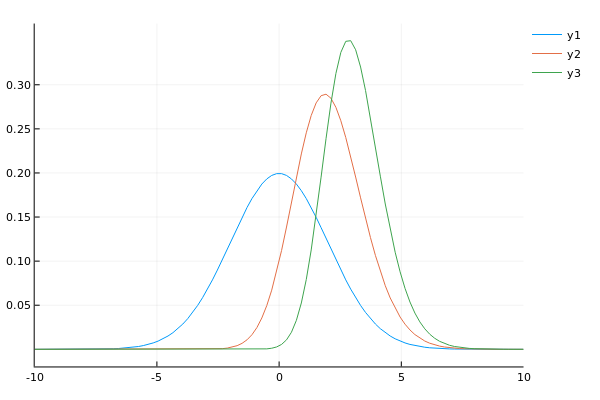
\includegraphics[scale=0.7]{images/order_stat_1_1.png}
\end{figure}

The original pdf is non-zero everywhere, therefore the distribution of the maximum has the same property. For increasing $N$, the distribution becomes (i) more peaky and (ii) moves to the right.

\todo{Is there some analytical result for $N\rightarrow \infty$?}


\subsection{General Order Statistics}

Let us now consider the statistics of $X_{(k)}$ with $1 < k < N$. We again consider the cdf first. We have

\bee
F_k(x) = P(X_{(k)}<x) = P(\text{k out of N RVs} < x) = {N \choose k} F_X^k(x) \left[ 1 - F_x(x) \right]^{N-k}
\eee

The cdf of the $k$-th order statistics means: (i) $k$ out of the total $N$ RVs must be smaller than $x$; this happens with probability $F_X^k(x)$ (since the RVs are independent) and (ii) the remaining $N-k$ RVs must be larger; this happens with probability $\left[ 1 - F_x(x) \right]^{N-k}$. It does not matter which RVs are smaller or larger than $x$; there are ${N \choose k}$ ways to select the RVs.

%%% Local Variables:
%%% mode: latex
%%% TeX-master: "journal"
%%% End:
